\section{Erklärung}
\subsection{Was ist Strom?}
\begin{frame}
\frametitle{Was ist Strom?}
\only<1>{
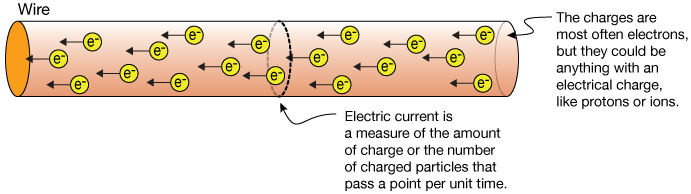
\includegraphics[width=\textwidth]{current}
}
\only<2->{
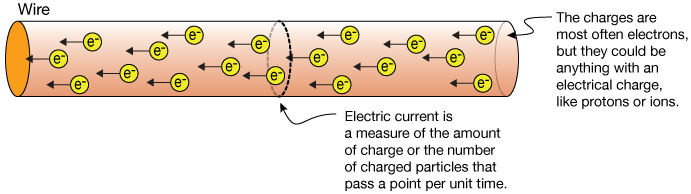
\includegraphics[width=0.7\textwidth]{current}\\[2ex]
\Large
\centering
$[C] = 6,240,000,000,000,000,000$ Elektronen\\[1ex]
\pause
$[A] = [C]/[s]$\\[1ex]
\pause
$I[A] = Q[C]/t[s]$
}
\note{
	Zeichne das Strom
}
\end{frame}

\tikzset{
	arrow/.style={
		->,
		thick,
		red
	}
}
\def\bruh{3ex}
\def\niger#1#2{{\normalsize\textbf{#1}} - #2}

\subsection{Was ist Spannung}
\begin{frame}
	\centering\Large Wissen sie?
\end{frame}
\begin{frame}
\frametitle{Was die Schulbücher uns über Spannung sagen}
\pause
\small
\begin{tikzpicture}
	\node (1) {\niger{Spannung}{der Anzahl an \textit{Joules} per Coloumb}};
	\pause
	\node[below=\bruh of 1] (2) {\niger{Joule}{eine Einheit von \textit{Energie}}};
	\draw[arrow] (1) -- (2);
	\pause

	\node[below=\bruh of 2] (3) {\niger{Energie}{die Kapazität \textit{Arbeit} zu tun}};
	\draw[arrow] (2) -- (3);
	\pause
	\node[below=\bruh of 3] (4) {\niger{Arbeit}{die Änderung in \textit{Energie}}};
	\draw[arrow] (3) -- (4);
	\pause
	\node[below=\bruh of 4] (5) {
\includegraphics[width=0.5\paperwidth]{images/understandable}};
	\draw[arrow] (4) -- (5);

\end{tikzpicture}
\centering


\note{
	Frage das Publikum,
	dann frage den Lehrer
	
	Weil in so eine Buch, finde ein Physik Buch. wir geschrieben dinge wie.

	Dann kommt der nachste klugkind und sagt, ja spannung ist wie Druck in eine Hose
}
\end{frame}

\begin{frame}
\frametitle{Die Schlauch Methaphor}
\pause
\centering
\Large Es wie druck in eine Schlauch
\begin{tikzpicture}
	\node at (current page.center) {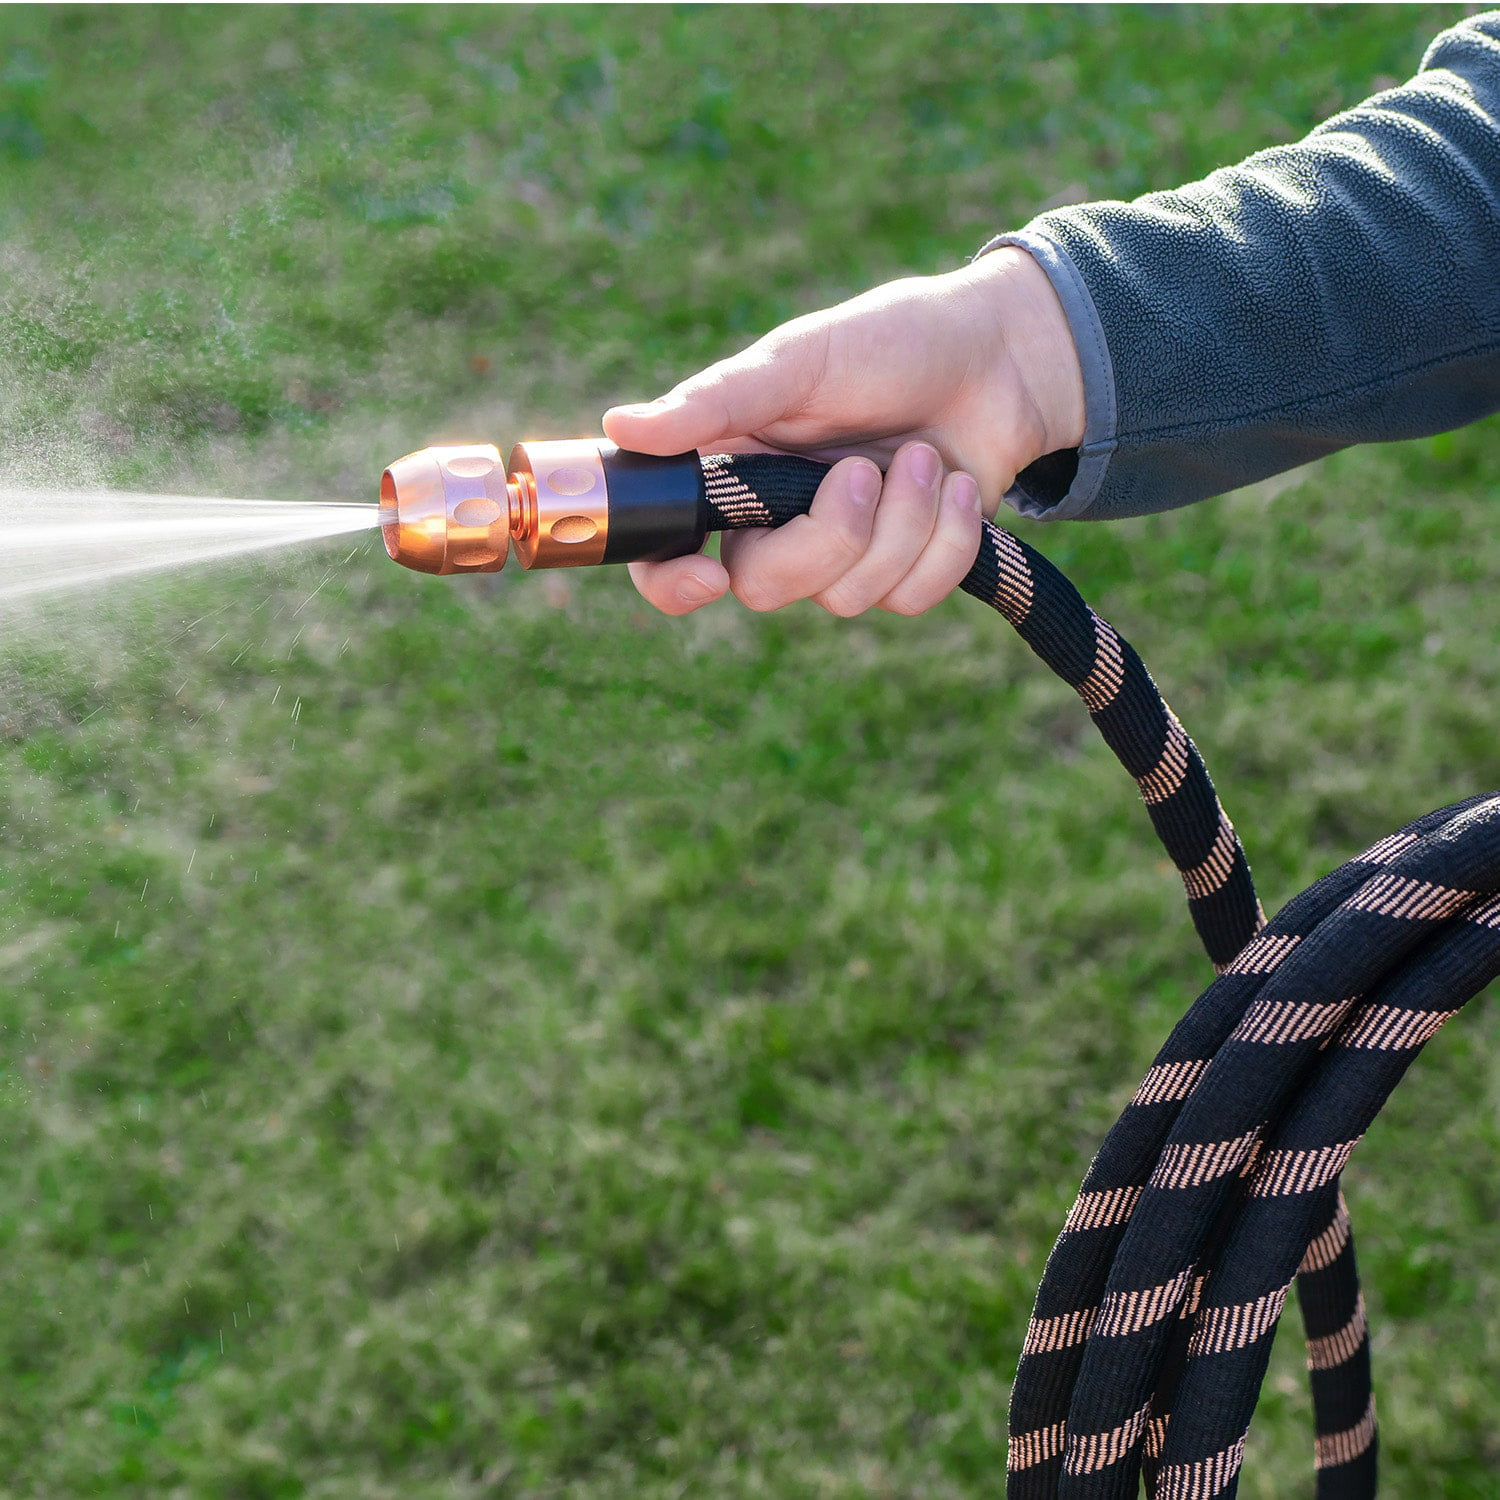
\includegraphics[width=0.7\textwidth]{images/hose}};
	\pause
	\node at (current page.center) {
\includegraphics[width=0.5\textwidth]{images/stop}};
\end{tikzpicture}

\end{frame}

\subsection{Nicht alle Elektronen sind gleich}
\begin{frameplain}
\centering\huge Nicht alle Elektronen sind gleich?
\end{frameplain}

\begin{frame}
	\frametitle{Spannung visualisiert}
	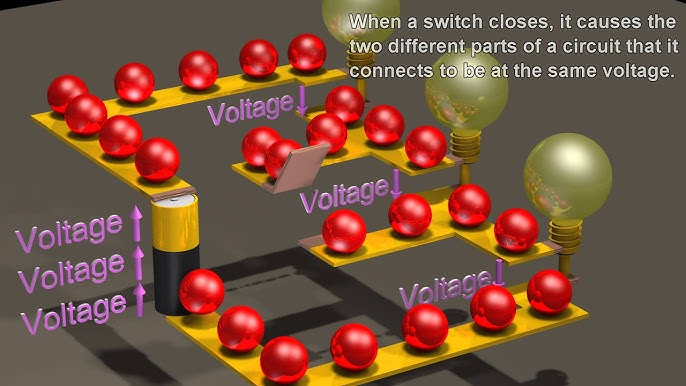
\includegraphics[width=\textwidth]{spannung}
\end{frame}

\section{Warum Wechselstrom}

\begin{frameplain}
\Large
Ok wir wissen warum wir Hochspannung benutzen, aber warum denn mit Wechselstrom?
\end{frameplain}

\subsection{Meet the Transformator}
\begin{frame}
	\frametitle{Meet the Transformator}
	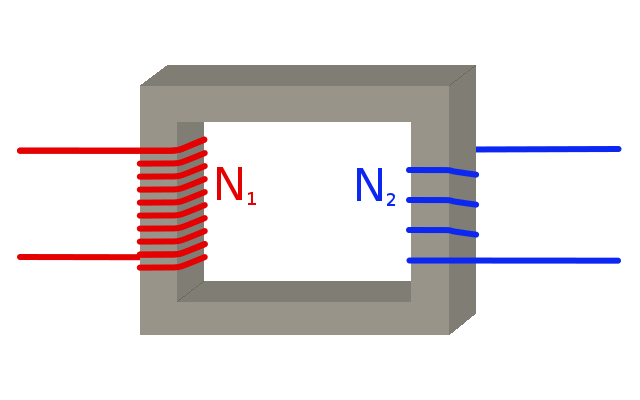
\includegraphics[width=\textwidth]{transformator}
\end{frame}

\subsection{Erklärung für der magnetische Feld}
\begin{frame}
	\frametitle{Relativität}
	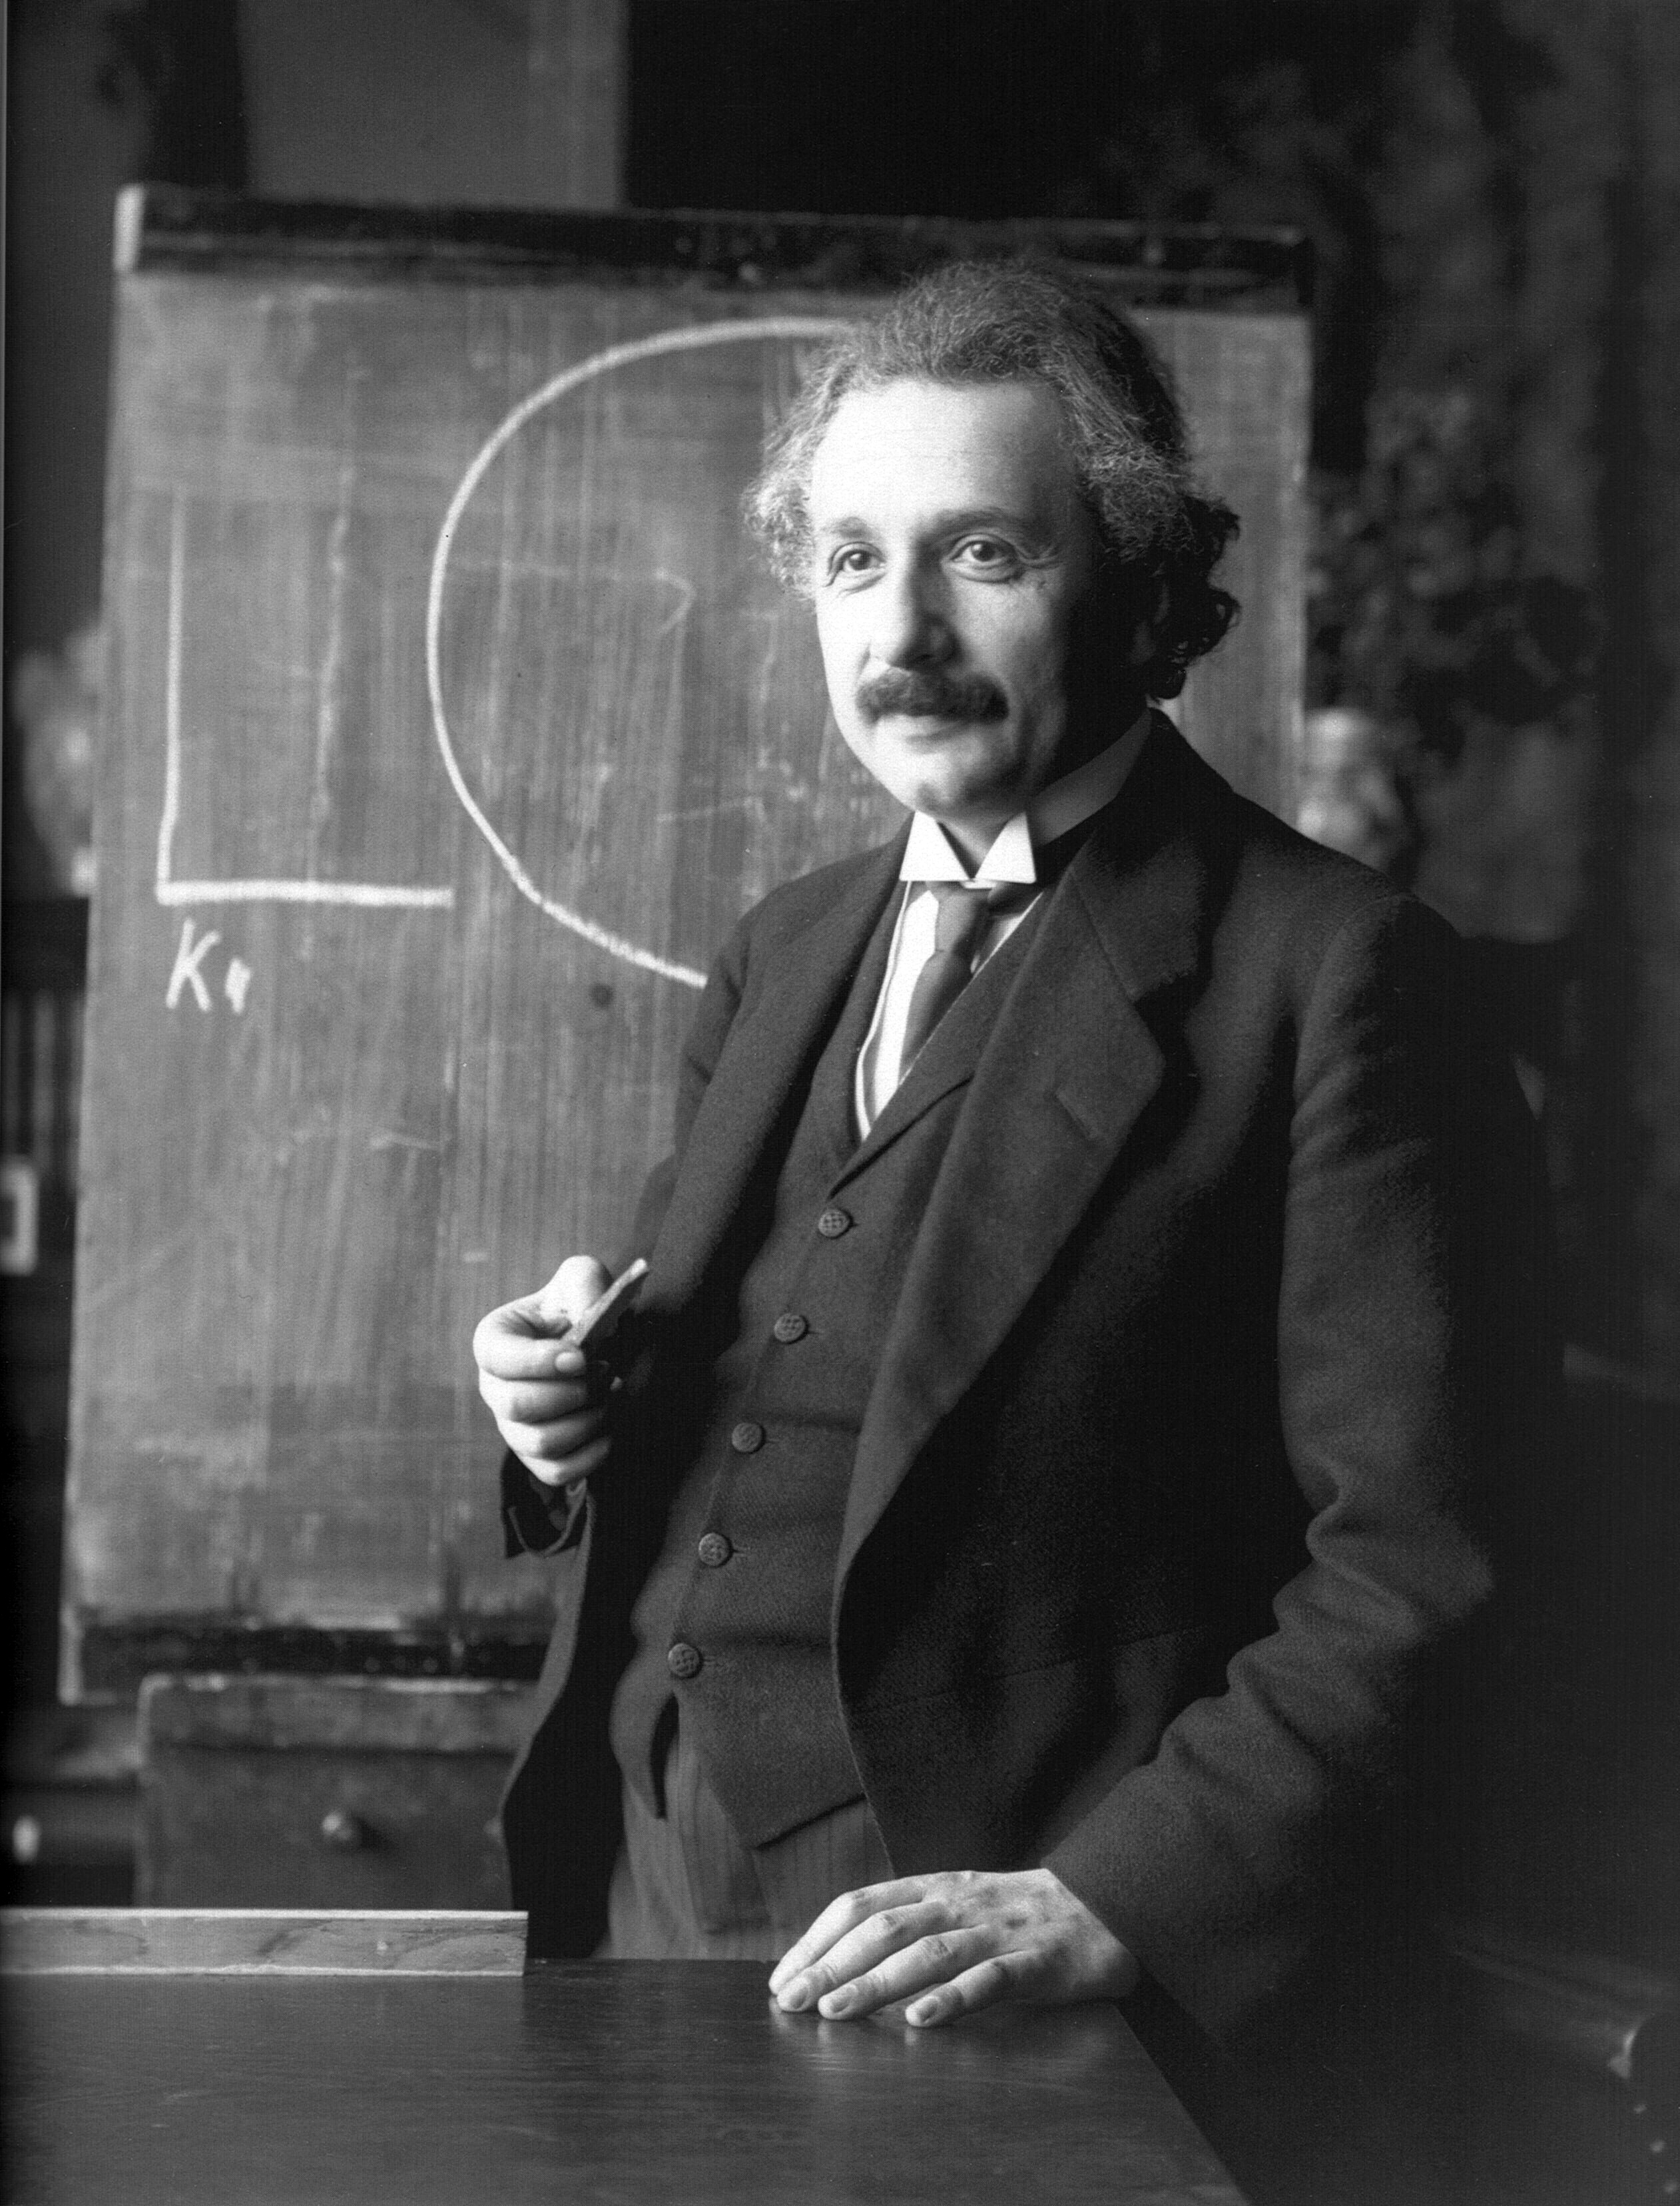
\includegraphics[width=0.3\textwidth]{einstein}\\
	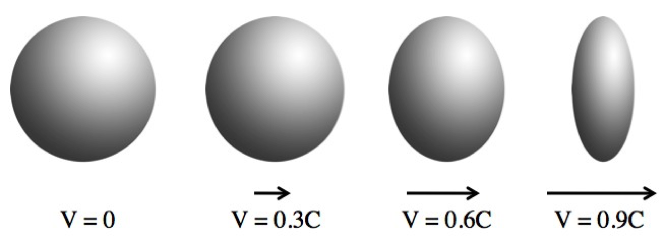
\includegraphics[width=\textwidth]{relativity}
\end{frame}

\begin{frame}
	\frametitle{Relativität}
	\centering
	\includegraphics[width=\textwidth]{alarmy}
\end{frame}

